\documentclass[aspectratio=169, 10pt]{beamer}
\usetheme[progressbar=frametitle, block=fill]{metropolis}

% --- SPRACHE & SCHRIFTEN ---
\usepackage{fontspec}
\usepackage[ngerman]{babel}
\usepackage{xcolor}
\usepackage{graphicx}
\usepackage{booktabs}
\usepackage{tabularx}
\usepackage{colortbl}
\usepackage{qrcode}
\usepackage{fontawesome5}

% --- TIKZ GRAFIKEN ---
\usepackage{tikz}
\usetikzlibrary{arrows.meta, positioning, calc, shapes.geometric, shadows, backgrounds}

% --- TCOLORBOX FÜR HIGHLIGHTS ---
\usepackage{tcolorbox}
\tcbuselibrary{skins, breakable}

% --- FARBSCHEMA (Passend zum Arbeitsblatt & Advanced Organizer) ---
\definecolor{primaryBlue}{RGB}{20, 50, 100}
\definecolor{lightBlue}{RGB}{242, 246, 252}
\definecolor{borderBlue}{RGB}{170, 195, 230}
\definecolor{accentOrange}{RGB}{220, 100, 30}
\definecolor{accentGreen}{RGB}{35, 130, 70}
\definecolor{accentRed}{RGB}{185, 45, 45}
\definecolor{subtleGray}{RGB}{248, 249, 251}
\definecolor{textDark}{RGB}{30, 35, 45}

% --- METROPOLIS DESIGN-ANPASSUNGEN ---
\setbeamercolor{palette primary}{bg=primaryBlue, fg=white}
\setbeamercolor{progress bar}{fg=accentOrange, bg=primaryBlue!20}
\setbeamercolor{title separator}{fg=accentOrange}
\setbeamercolor{progress bar in head/foot}{fg=accentOrange, bg=primaryBlue!20}
\setbeamercolor{progress bar in section page}{fg=accentOrange, bg=primaryBlue!20}
\setbeamercolor{frametitle}{bg=primaryBlue, fg=white}
\setbeamercolor{background canvas}{bg=white}
\setbeamercolor{normal text}{fg=textDark}
\setbeamercolor{block title}{bg=primaryBlue, fg=white}
\setbeamercolor{block body}{bg=lightBlue, fg=textDark}
\setbeamercolor{block title alerted}{bg=accentOrange, fg=white}
\setbeamercolor{block body alerted}{bg=accentOrange!10, fg=textDark}
\setbeamercolor{block title example}{bg=accentGreen, fg=white}
\setbeamercolor{block body example}{bg=accentGreen!10, fg=textDark}

% Eigene Box-Stile
\tcbset{
    modernCard/.style={
        enhanced,
        boxrule=0.8pt,
        arc=3mm,
        left=6pt, right=6pt, top=6pt, bottom=6pt,
        boxsep=0pt,
        fonttitle=\bfseries\footnotesize,
        coltitle=white
    },
    rousseauNature/.style={
        modernCard,
        colframe=accentGreen,
        colback=accentGreen!6,
        coltitle=white
    },
    rousseauCulture/.style={
        modernCard,
        colframe=accentRed,
        colback=accentRed!6,
        coltitle=white
    },
    infoCard/.style={
        modernCard,
        colframe=primaryBlue,
        colback=lightBlue,
        coltitle=white
    },
    alertCard/.style={
        modernCard,
        colframe=accentOrange,
        colback=accentOrange!8,
        coltitle=white
    }
}

% Metadaten
\title{Entfremdender Luxus oder nackte Notwendigkeit?}
\subtitle{Arnold Gehlens anthropologische Begründung der Kultur (1940)}
\author{Herr Dayi · Philosophie Q1}
\date{Themenfeld: Anthropologie}

\begin{document}

% -------------------------------------------------------------
% FOLIE 1: TITEL
% -------------------------------------------------------------
\begin{frame}[plain]
    \maketitle
\end{frame}

% -------------------------------------------------------------
% FOLIE 2: EINSTIEG & REAKTIVIERUNG ROUSSEAU
% -------------------------------------------------------------
\begin{frame}{Reaktivierung: Rousseaus Seelenkräfte im Text-Check}
    \vspace{-0.25cm}
    \begin{columns}[T]
        \begin{column}{0.68\textwidth}
            \begin{tcolorbox}[infoCard, title={\faTasks\ Blitz-Auftrag (Partnerarbeit · 3–4 Minuten)}]
                \footnotesize
                Ordnet die 4 Schlüsselbegriffe in das Schaubild ein und vollzieht die Pfeile nach:\\
                \begin{center}
                    \textbf{Vernunft} $\cdot$ \textbf{Eigenliebe} $\cdot$ \textbf{Mitleid} $\cdot$ \textbf{Selbstliebe}
                \end{center}
            \end{tcolorbox}

            \vspace{0.12cm}
            \begin{tcolorbox}[alertCard, title={\faSearch\ Text-Spurensuche (Zeilenangaben vom Arbeitsblatt)}]
                \scriptsize
                \begin{itemize}\setlength{\itemsep}{2pt}
                    \item \textbf{Pfeil 1 (Z. 63–64):} Welche Kraft \textit{erzeugt \& verstärkt} die Eigenliebe?
                    \item \textbf{Pfeil 2 (Z. 67–72):} Warum \textit{erstickt} der gebildete Philosoph das Mitleid?
                    \item \textbf{Pfeil 3 (Z. 77–80):} Warum \textit{mäßigt \& zügelt} das Mitleid die Selbstliebe?
                \end{itemize}
            \end{tcolorbox}
        \end{column}

        \begin{column}{0.30\textwidth}
            \centering
            \begin{tcolorbox}[enhanced, colframe=primaryBlue, colback=white, arc=3mm, boxrule=0.8pt, title={\faLaptopCode\ Digitale Übung}, fonttitle=\scriptsize\bfseries]
                \centering
                \qrcode[height=2.3cm]{https://herrdayi.github.io/Gehlen/reaktivierung.html}
                \\[0.15cm]
                \tiny\texttt{herrdayi.github.io/Gehlen/}\\[-0.05cm]
                \tiny\texttt{reaktivierung.html}
                \\[0.12cm]
                \scriptsize\faHandPointer\ \textbf{Jetzt am Tablet lösen!}
            \end{tcolorbox}
        \end{column}
    \end{columns}
\end{frame}

% -------------------------------------------------------------
% FOLIE 3: HEUTIGER ABLAUF
% -------------------------------------------------------------
\begin{frame}{Heutiger Fahrplan (Doppelstunde · 90 Minuten)}
    \vspace{-0.15cm}
    \begin{columns}[T]
        \begin{column}{0.64\textwidth}
            \begin{enumerate}\setlength{\itemsep}{3pt}\footnotesize
                \item \textbf{Reaktivierung \& Verortung} (10 min)\\
                {\scriptsize Klärung Rousseau (\textit{amour de soi}) \& Eintragung im Advanced Organizer}
                \item \textbf{Kognitiver Konflikt} (10 min)\\
                {\scriptsize Das Gedankenexperiment: Der nackte Mensch im Winterwald}
                \item \textbf{Methoden-Check: Reziprokes Lesen} (10 min)\\
                {\scriptsize 4 Rollen zur Texterschließung \& digitaler Methodenkoffer (TaskCards)}
                \item \textbf{Arbeitsphase: Arnold Gehlen} (30 min)\\
                {\scriptsize Partnerarbeit mit Rollenwechsel, Arbeitsblatt \& Lernumgebung}
                \item \textbf{Sicherung \& Systematisierung} (15 min)\\
                {\scriptsize Gehlens Argumentationsgang als Wirkungsgefüge (Schaubild)}
                \item \textbf{Synthese \& Ausblick} (15 min)\\
                {\scriptsize Methodenreflexion, Verortung im AO \& Problemüberhang zu Freud}
            \end{enumerate}
        \end{column}
        
        \begin{column}{0.32\textwidth}
            \centering
            \begin{tcolorbox}[infoCard, title={\faClock\ Zeitmanagement}]
                \centering\scriptsize
                \textbf{90 Minuten Fokus}\\[0.1cm]
                \faUsers\ Partnerarbeit (PA)\\
                \faTablet*\ Digitale Hilfen (AO \& Gehlen)\\
                \faBrain\ Philosophische Urteilskraft
            \end{tcolorbox}
            \vspace{0.15cm}
            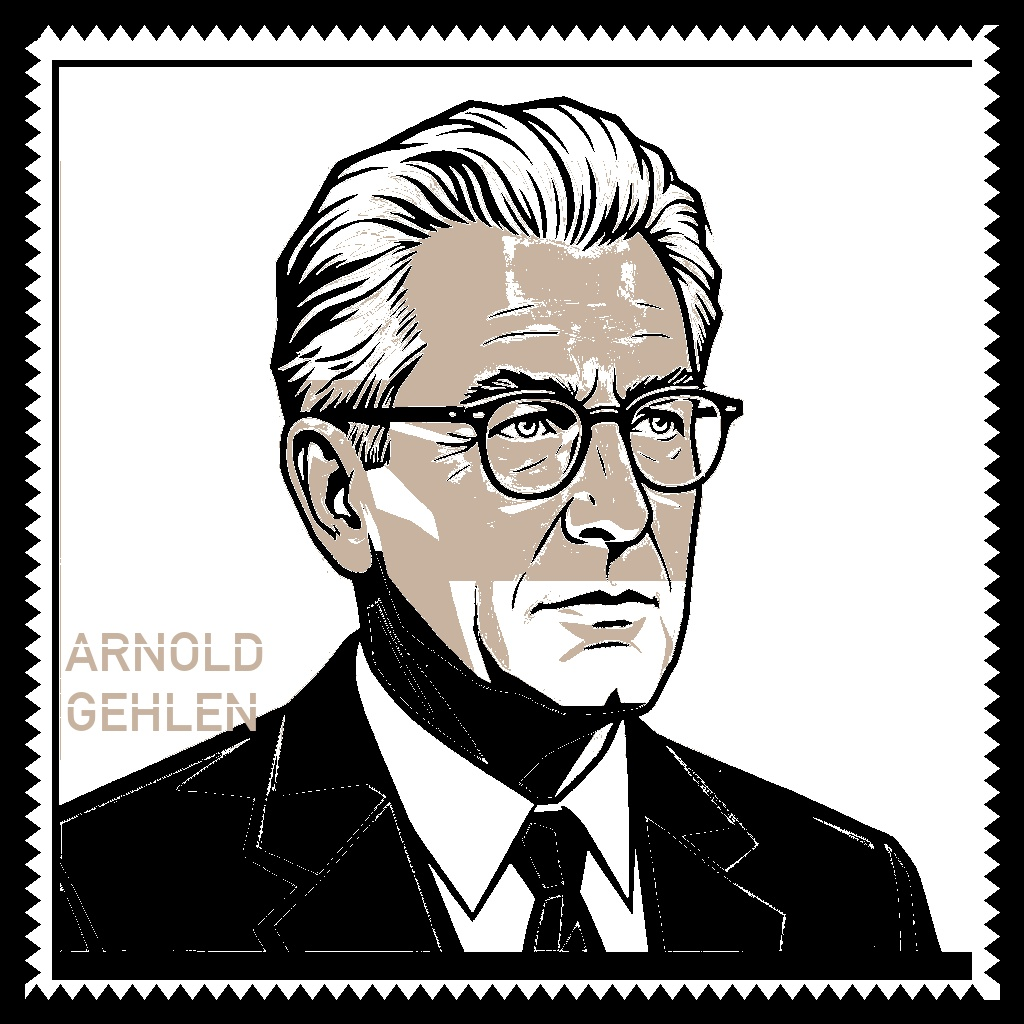
\includegraphics[width=0.55\textwidth]{gehlen.jpeg}
        \end{column}
    \end{columns}
\end{frame}

% -------------------------------------------------------------
% FOLIE 4: ADVANCED ORGANIZER (AO)
% -------------------------------------------------------------
\begin{frame}{Der Advanced Organizer: Braucht der Mensch Kultur?}
    \vspace{-0.2cm}
    \begin{columns}[T]
        \begin{column}{0.67\textwidth}
            \begin{tcolorbox}[infoCard, title={\faCompass\ Das Spektrum unserer Unterrichtsreihe}]
                \vspace{0.1cm}
                \begin{tikzpicture}[xscale=0.88, yscale=0.8]
                    % Skala
                    \draw[line width=2pt, primaryBlue] (0, 0) -- (6.8, 0);
                    
                    % Pol A
                    \node[draw=primaryBlue, fill=lightBlue, rounded corners=3pt, font=\scriptsize\bfseries, align=center] at (0, 0.9) 
                        {\textbf{POL A}\\\textcolor{primaryBlue}{Kultur als Notwendigkeit}\\{\tiny Schutz, Lebensbedingung}};
                    \draw[primaryBlue, line width=1.5pt] (0, 0.2) -- (0, -0.2);

                    % Pol B
                    \node[draw=accentRed, fill=accentRed!8, rounded corners=3pt, font=\scriptsize\bfseries, align=center] at (6.8, 0.9) 
                        {\textbf{POL B}\\\textcolor{accentRed}{Kultur als Verhängnis}\\{\tiny Entfremdung, Korruption}};
                    \draw[accentRed, line width=1.5pt] (6.8, 0.2) -- (6.8, -0.2);

                    % Verortung Rousseau
                    \node[draw=accentRed, fill=white, rounded corners=2pt, font=\tiny\bfseries, text=accentRed] at (6.4, -0.6) 
                        {\faUserCheck\ J.-J. Rousseau};

                    % Verortung Gehlen Fragezeichen
                    \node[draw=primaryBlue, dashed, fill=white, rounded corners=2pt, font=\tiny\bfseries, text=primaryBlue] at (0.4, -0.6) 
                        {\faQuestionCircle\ Arnold Gehlen?};
                \end{tikzpicture}
            \end{tcolorbox}
            \vspace{0.1cm}
            \footnotesize
            \faArrowCircleRight\ \textbf{Arbeitsauftrag:} Öffnet den Advanced Organizer auf eurem Tablet und verortet Rousseaus These über die Selbstliebe am Pol B!
        \end{column}

        \begin{column}{0.31\textwidth}
            \centering
            \begin{tcolorbox}[enhanced, colframe=primaryBlue, colback=white, arc=3mm, boxrule=0.8pt, title={\faQrcode\ Advanced Organizer}, fonttitle=\scriptsize\bfseries]
                \centering
                \qrcode[height=2.3cm]{https://herrdayi.github.io/AO/}
                \\[0.15cm]
                \scriptsize\texttt{herrdayi.github.io/AO}
            \end{tcolorbox}
        \end{column}
    \end{columns}
\end{frame}

% -------------------------------------------------------------
% FOLIE 5: KOGNITIVER KONFLIKT / DAS GEDANKENEXPERIMENT
% -------------------------------------------------------------
\begin{frame}{Kognitive Dissonanz: Der nackte Mensch im Winterwald}
    \vspace{-0.3cm}
    \begin{columns}[T]
        \begin{column}{0.48\textwidth}
            \begin{tcolorbox}[rousseauNature, title={\faQuestionCircle\ Rousseaus Naturideal}]
                \begin{itemize}\setlength{\itemsep}{1.5pt}\footnotesize
                    \item Der Mensch ist im Naturzustand autark.
                    \item Die Natur stillt alle seine Bedürfnisse.
                    \item \textit{amour de soi} genügt zum glücklichen Leben.
                    \item \textbf{These:} Kultur ist überflüssiger Luxus.
                \end{itemize}
            \end{tcolorbox}
        \end{column}

        \begin{column}{0.48\textwidth}
            \begin{tcolorbox}[rousseauCulture, title={\faBolt\ Das biologische Gedankenexperiment}]
                \textbf{Ein nackter Mensch im Winterwald (-10°C):}
                \begin{itemize}\setlength{\itemsep}{1.5pt}\footnotesize
                    \item \textbf{Kein Fell:} Tödliche Unterkühlung
                    \item \textbf{Keine Krallen / Reißzähne:} Wehrlos
                    \item \textbf{Fluchtuntauglich:} Weder schnell noch kletterbegabt
                    \item \textbf{Biologisches Verdikt:} Nach Stunden tot!
                \end{itemize}
            \end{tcolorbox}
        \end{column}
    \end{columns}

    \vspace{0.15cm}
    \begin{tcolorbox}[alertCard, title={\faExclamationTriangle\ Die Leitfrage unserer Doppelstunde}]
        \centering\small\bfseries
        \glqq Entfremdender Luxus oder nackte Notwendigkeit:\\
        Warum kann der Mensch ohne Kultur biologisch gar nicht überleben?\grqq
    \end{tcolorbox}
\end{frame}

% -------------------------------------------------------------
% FOLIE 6: METHODISCHER BAUSTEIN: REZIPROKES LESEN
% -------------------------------------------------------------
\begin{frame}{Texterschließungsmethode: Reziprokes Lesen (4 Rollen)}
    \vspace{-0.25cm}
    \begin{columns}[T]
        \begin{column}{0.48\textwidth}
            \begin{tcolorbox}[modernCard, colframe=primaryBlue, colback=lightBlue, title={\faQuestionCircle\ 1. Der Frager}]
                \footnotesize
                \textbf{Aufgabe:} Stellt inhaltliche Fragen zum Sinnabschnitt.\\[2pt]
                \textit{Satzstarter:} \glqq Warum behauptet Gehlen, dass...?\grqq
            \end{tcolorbox}
            \vspace{0.12cm}
            \begin{tcolorbox}[modernCard, colframe=accentGreen, colback=accentGreen!8, title={\faAlignLeft\ 3. Der Zusammenfasser}]
                \footnotesize
                \textbf{Aufgabe:} Bringt den Kern in 1–2 Sätzen auf den Punkt.\\[2pt]
                \textit{Satzstarter:} \glqq Im Kern geht es darum, dass...\grqq
            \end{tcolorbox}
        \end{column}

        \begin{column}{0.48\textwidth}
            \begin{tcolorbox}[modernCard, colframe=accentOrange, colback=accentOrange!8, title={\faSearch\ 2. Der Klärer}]
                \footnotesize
                \textbf{Aufgabe:} Spürt Fachwörter \& unklare Passagen auf.\\[2pt]
                \textit{Satzstarter:} \glqq Der Begriff X bedeutet im Kontext...\grqq
            \end{tcolorbox}
            \vspace{0.12cm}
            \begin{tcolorbox}[modernCard, colframe=primaryBlue!70, colback=primaryBlue!6, title={\faLightbulb\ 4. Der Vorhersager}]
                \footnotesize
                \textbf{Aufgabe:} Mutmaßt über die Fortführung des Textes.\\[2pt]
                \textit{Satzstarter:} \glqq Gehlen wird als Nächstes zeigen, dass...\grqq
            \end{tcolorbox}
        \end{column}
    \end{columns}

    \vspace{0.15cm}
    \centering\footnotesize
    \textbf{Partnerarbeit (PA):} Teilt die 4 Rollen auf (2 Rollen pro Person) und tauscht nach jedem Textabschnitt!
\end{frame}

% -------------------------------------------------------------
% FOLIE 7: TASKCARDS METHODENKOFFER
% -------------------------------------------------------------
\begin{frame}{Methodenkoffer: Texterschließungsmethoden (TaskCards)}
    \vspace{-0.2cm}
    \begin{columns}[T]
        \begin{column}{0.68\textwidth}
            \begin{tcolorbox}[infoCard, title={\faThLarge\ Digitales Methoden-Board (Philosophie Q1 · Herr Dayi)}]
                \footnotesize
                Auf unserem TaskCards-Board findet ihr passgenaue Hilfekarten:
                \begin{itemize}\setlength{\itemsep}{3pt}
                    \item \textbf{Reziprokes Lesen:} Rollenkarten mit konkreten Satzanfängen für den Dialog zu zweit.
                    \item \textbf{5-Schritt-Lesemethode:} Strukturierte Anleitung (Überfliegen $\rightarrow$ Fragen $\rightarrow$ Lesen $\rightarrow$ Zusammenfassen $\rightarrow$ Rekapitulieren).
                    \item \textbf{Methoden-Vergleich:} Wann eignet sich welche Lesestrategie?
                \end{itemize}
                \vspace{0.1cm}
                \textit{\faInfoCircle\ Nutzt das Board während der Textarbeit als Stütze auf eurem Gerät.}
            \end{tcolorbox}
        \end{column}

        \begin{column}{0.28\textwidth}
            \centering
            \begin{tcolorbox}[enhanced, colframe=primaryBlue, colback=white, arc=3mm, boxrule=0.8pt, title={\faQrcode\ TaskCards Board}]
                \centering
                \qrcode[height=2.3cm]{https://www.taskcards.de/\#/board/4fff3dd6-9170-4de7-8ea0-33706e93ccc2/view}
                \\[0.15cm]
                \tiny\texttt{taskcards.de/board/...}
            \end{tcolorbox}
        \end{column}
    \end{columns}
\end{frame}

% -------------------------------------------------------------
% FOLIE 8: ERARBEITUNG: ARNOLD GEHLEN
% -------------------------------------------------------------
\begin{frame}{Arbeitsphase: Arnold Gehlens Kulturanthropologie (1940)}
    \vspace{-0.2cm}
    \begin{columns}[T]
        \begin{column}{0.7\textwidth}
            \begin{tcolorbox}[infoCard, title={\faTasks\ Arbeitsaufträge (Partnerarbeit · 30 Minuten)}]
                \footnotesize
                \textbf{Material:} Arbeitsblatt (Textauszug Gehlen: \textit{Der Mensch}) \& Tablet
                \begin{enumerate}\setlength{\itemsep}{4pt}
                    \item \textbf{Aufgabe 1 (PA):} Erschließt Gehlens anthropologischen Befund des \textbf{Mängelwesens}. Arbeitet seine biologischen Defizite präzise heraus.
                    \item \textbf{Aufgabe 2 (PA):} Strukturiert Gehlens Argumentation in einem \textbf{Schaubild}. Verknüpft die 5 Begriffe:
                    \begin{center}
                        \textbf{Mängelwesen} $\cdot$ \textbf{Weltoffenheit} $\cdot$ \textbf{Handeln} $\cdot$ \textbf{Kultur} $\cdot$ \textbf{Institutionen}
                    \end{center}
                    \textit{Tipp: Beschriftet alle Pfeile mit Verben (z.\,B. kompensiert, erfordert)!}
                    \item \textbf{Schnelldenker:} Erklärt den Fall der Wolfskinder Amala \& Kamala anhand von Gehlens Modell.
                \end{enumerate}
            \end{tcolorbox}
        \end{column}

        \begin{column}{0.28\textwidth}
            \centering
            \begin{tcolorbox}[enhanced, colframe=primaryBlue, colback=white, arc=3mm, boxrule=0.8pt, title={\faLaptopCode\ Lernumgebung}]
                \centering
                \qrcode[height=2.2cm]{https://herrdayi.github.io/Gehlen/}
                \\[0.15cm]
                \tiny\texttt{herrdayi.github.io/Gehlen}
                \\[0.1cm]
                \scriptsize\faLightbulb\ \textbf{Hilfe zu Aufgabe 2:}\\
                Interaktiver Beziehungs- \& Verben-Finder!
            \end{tcolorbox}
        \end{column}
    \end{columns}
\end{frame}

% -------------------------------------------------------------
% FOLIE 9: DAS ARBEITSBLATT IM ÜBERBLICK
% -------------------------------------------------------------
\begin{frame}{Das Arbeitsblatt im Überblick}
    \begin{columns}[c]
        \begin{column}{0.48\textwidth}
            \centering
            \begin{tcolorbox}[enhanced, colframe=primaryBlue, colback=white, boxrule=0.8pt, arc=2mm, left=2pt, right=2pt, top=2pt, bottom=2pt, title={\scriptsize\textbf{Seite 1: Textarbeit \& Mängelwesen}}]
                \centering
                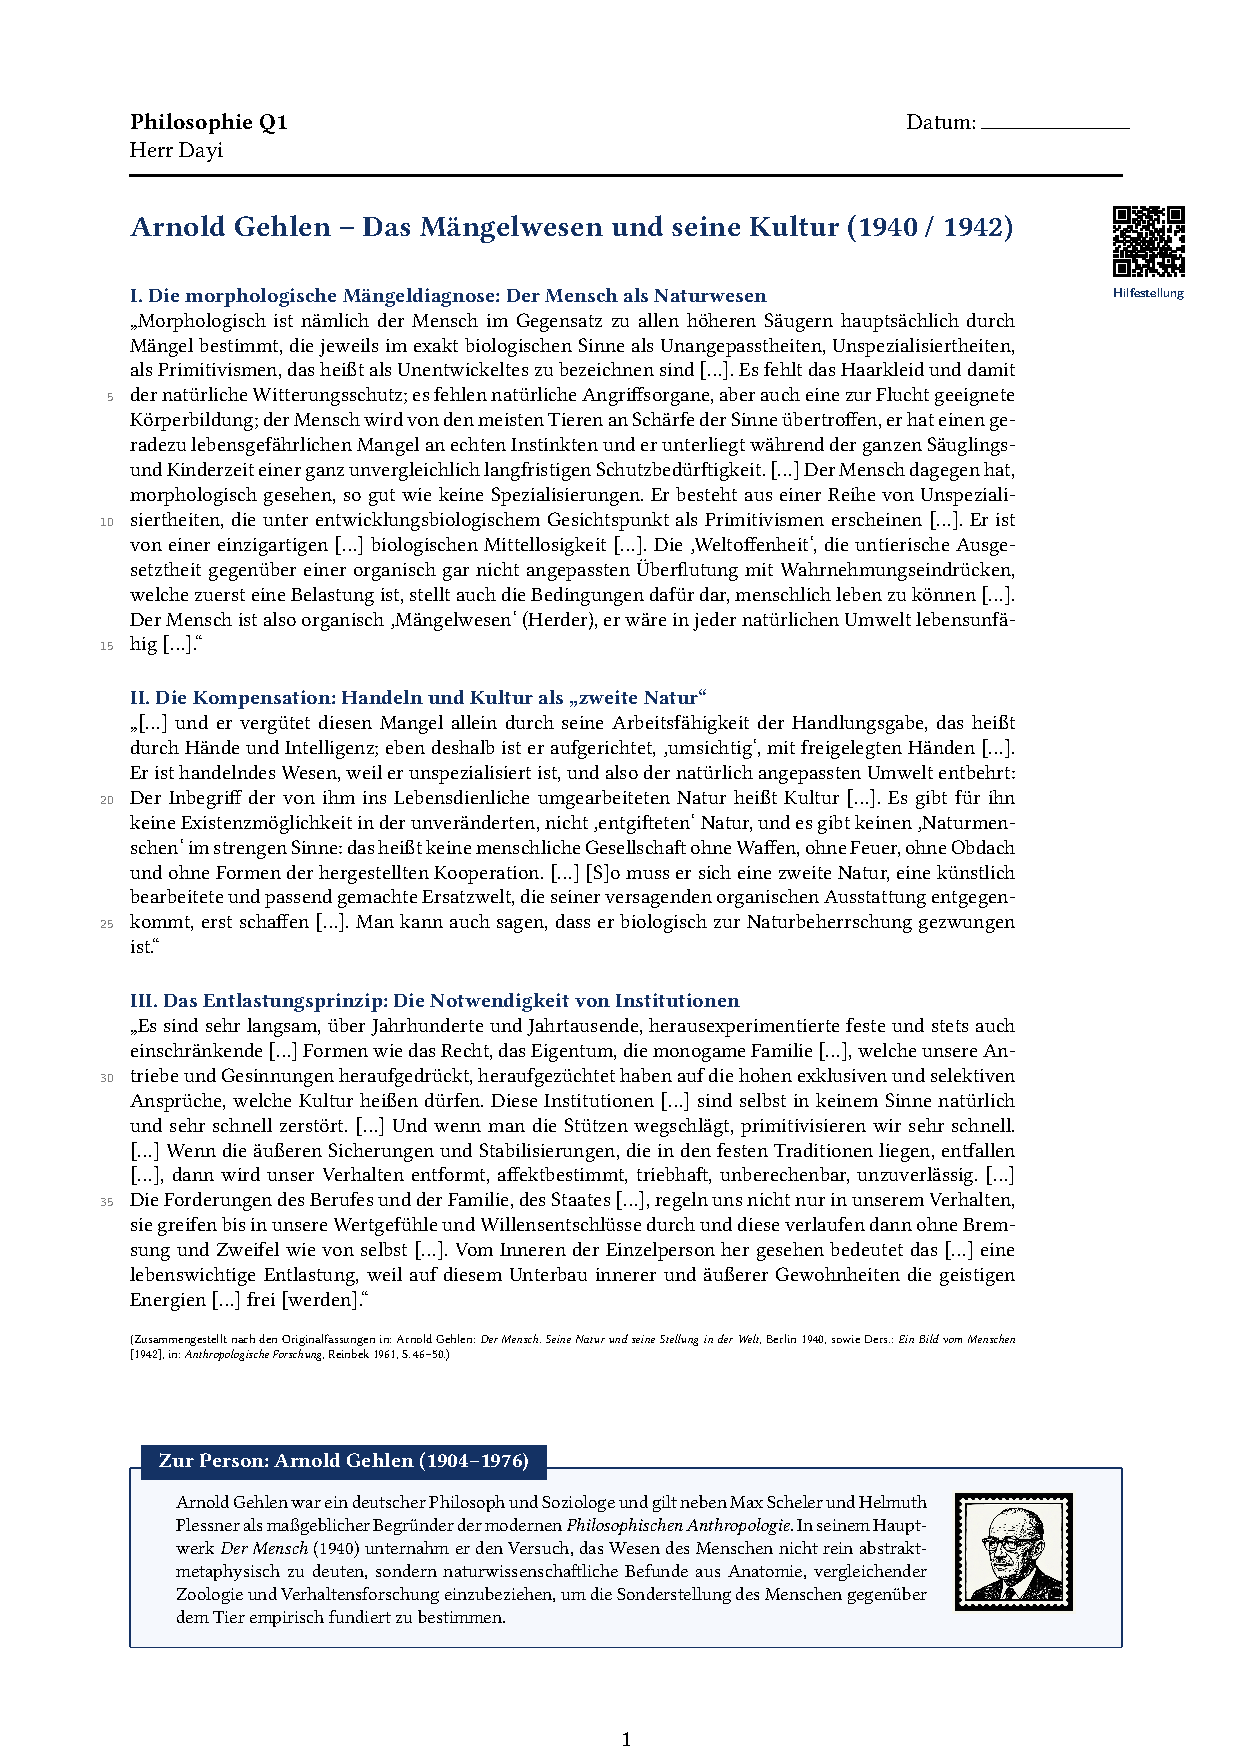
\includegraphics[page=1, height=0.62\textheight, keepaspectratio]{AB.pdf}
            \end{tcolorbox}
        \end{column}

        \begin{column}{0.48\textwidth}
            \centering
            \begin{tcolorbox}[enhanced, colframe=primaryBlue, colback=white, boxrule=0.8pt, arc=2mm, left=2pt, right=2pt, top=2pt, bottom=2pt, title={\scriptsize\textbf{Seite 2: Schaubild \& Schnelldenker}}]
                \centering
                \includegraphics[page=2, height=0.62\textheight, keepaspectratio]{AB.pdf}
            \end{tcolorbox}
        \end{column}
    \end{columns}
    \vspace{0.15cm}
    \centering\footnotesize
    \textbf{Fokus auf Seite 2:} Zeichnet euer individuelles Schaubild mit aussagekräftigen Pfeilverknüpfungen!
\end{frame}

% -------------------------------------------------------------
% FOLIE 10: SICHERUNG: GEHLENS ANTHROPOLOGISCHES WIRKUNGSGEFÜGE
% -------------------------------------------------------------
\begin{frame}{Sicherung: Gehlens anthropologisches Wirkungsgefüge}
    \vspace{-0.25cm}
    \begin{center}
    \begin{tikzpicture}[
        concept/.style={
            rectangle, rounded corners=4pt, draw=primaryBlue, fill=lightBlue,
            line width=1.1pt, text width=2.35cm, minimum height=1.75cm,
            align=center, font=\footnotesize, inner sep=2.5pt
        },
        arrow/.style={
            -{Stealth[scale=1.1]}, line width=1.3pt, color=primaryBlue
        },
        arrowlabel/.style={
            font=\tiny\bfseries, text=accentOrange, fill=white, inner sep=1.2pt, rounded corners=2pt, draw=accentOrange!40
        }
    ]
        \node[concept] (c1) {\textbf{1. Mängelwesen}\\\scriptsize Organisch unfertig, mittellos, instinktreduziert};
        \node[concept, right=0.38cm of c1] (c2) {\textbf{2. Weltoffenheit}\\\scriptsize Reizüberflutung, unbestimmte Umwelt};
        \node[concept, right=0.38cm of c2] (c3) {\textbf{3. Handeln}\\\scriptsize Zweckgerichtete Naturbeherrschung};
        \node[concept, right=0.38cm of c3] (c4) {\textbf{4. Kultur}\\\scriptsize \glqq Zweite Natur\grqq, Sprache, Technik};
        \node[concept, right=0.38cm of c4] (c5) {\textbf{5. Institutionen}\\\scriptsize Recht, Staat, Sitten, feste Ordnungen};

        % Pfeile Kette
        \draw[arrow] ($(c1.east)+(0,0.15)$) -- node[midway, above=1.5pt, arrowlabel] {erzeugt} ($(c2.west)+(0,0.15)$);
        \draw[arrow] ($(c2.east)+(0,0.15)$) -- node[midway, above=1.5pt, arrowlabel] {zwingt zu} ($(c3.west)+(0,0.15)$);
        \draw[arrow] ($(c3.east)+(0,0.15)$) -- node[midway, above=1.5pt, arrowlabel] {schafft} ($(c4.west)+(0,0.15)$);
        \draw[arrow] ($(c4.east)+(0,0.15)$) -- node[midway, above=1.5pt, arrowlabel] {stabilisiert} ($(c5.west)+(0,0.15)$);

        % Großer Entlastungsbogen
        \draw[-{Stealth[scale=1.3]}, line width=1.6pt, color=accentGreen] 
            (c5.south) -- ++(0,-0.55) -| node[pos=0.25, below=1pt, font=\scriptsize\bfseries, text=accentGreen] 
            {\textbf{DAS ENTLASTUNGSPRINZIP:} Verhaltenssicherheit \& Schutz vor Reizüberflutung} (c1.south);
    \end{tikzpicture}
    \end{center}

    \vspace{-0.1cm}
    \begin{columns}[T]
        \begin{column}{0.48\textwidth}
            \begin{tcolorbox}[infoCard, title={\scriptsize\textbf{Kompensation \& \glqq Zweite Natur\grqq}}]
                \tiny
                Kultur ist für Gehlen kein Luxus, sondern die vom Menschen selbst geschaffene biologische Ersatzwelt zur Selbsterhaltung.
            \end{tcolorbox}
        \end{column}
        \begin{column}{0.48\textwidth}
            \begin{tcolorbox}[modernCard, colframe=accentGreen, colback=accentGreen!8, title={\scriptsize\textbf{Die Funktion der Institutionen}}]
                \tiny
                Institutionen entlasten von ständigen Entscheidungen, bändigen Triebimpulse und sichern das Überleben im Kollektiv.
            \end{tcolorbox}
        \end{column}
    \end{columns}
\end{frame}

% -------------------------------------------------------------
% FOLIE 11: METHODENREFLEXION
% -------------------------------------------------------------
\begin{frame}{Metakognition: Methodenreflexion Texterschließung}
    \vspace{-0.2cm}
    \begin{columns}[T]
        \begin{column}{0.48\textwidth}
            \begin{tcolorbox}[modernCard, colframe=primaryBlue, colback=lightBlue, title={\faUsers\ Reziprokes Lesen (heute erprobt)}]
                \textbf{Erfahrungen \& Stärken:}
                \begin{itemize}\setlength{\itemsep}{2pt}\scriptsize
                    \item \textbf{Aktive Kooperation:} Niemand liest passiv \glqq über den Text hinweg\grqq.
                    \item \textbf{Begriffspräzision:} Unklare Fachbegriffe (\textit{Weltoffenheit, Mängelwesen}) werden sofort im Dialog geklärt.
                    \item \textbf{Rollenbewusstsein:} Formulierung konkreter Leitfragen zwingt zum Mitdenken.
                    \item \textit{Grenze:} Zeitintensiver als stilles Überfliegen.
                \end{itemize}
            \end{tcolorbox}
        \end{column}

        \begin{column}{0.48\textwidth}
            \begin{tcolorbox}[modernCard, colframe=subtleGray!40!black, colback=subtleGray, title={\faBookOpen\ 5-Schritt-Lesemethode (SQ3R)}]
                \textbf{Vergleich \& Einsatzbereich:}
                \begin{itemize}\setlength{\itemsep}{2pt}\scriptsize
                    \item \textbf{Strukturierter Leitfaden:} Ideal für die eigenständige Vorbereitung \& Klausur.
                    \item \textbf{Gesamtüberblick:} Stark bei langen Sachtexten mit Gliederungsüberschriften.
                    \item \textit{Grenze:} In Einzelarbeit besteht die Gefahr, schwierige philosophische Passagen zu überspringen.
                \end{itemize}
            \end{tcolorbox}
        \end{column}
    \end{columns}

    \vspace{0.2cm}
    \begin{tcolorbox}[alertCard, title={\faComments\ Reflexionsimpuls für das Plenum}]
        \centering\footnotesize
        \textbf{Frage:} Welche der 4 Rollen hat euch heute am meisten dabei geholfen, Gehlens dichten Textabschnitt zu entschlüsseln – und warum?
    \end{tcolorbox}
\end{frame}

% -------------------------------------------------------------
% FOLIE 12: ABSCHLUSS, AO-RÜCKBLICK & PROBLEMÜBERHANG ZU FREUD
% -------------------------------------------------------------
\begin{frame}{Synthese im AO \& Problemüberhang zur nächsten Stunde}
    \vspace{-0.2cm}
    \begin{columns}[T]
        \begin{column}{0.65\textwidth}
            \begin{tcolorbox}[infoCard, title={\faCheckCircle\ Sicherung im Advanced Organizer}]
                \footnotesize
                \textbf{Gehlens Verortung an Pol A:}\\
                Kultur ist kein entfremdender Luxus (Rousseau), sondern \textbf{existenzielle Lebensbedingung}. Ohne Kultur und Institutionen ist der Mensch lebensunfähig.
            \end{tcolorbox}

            \vspace{0.15cm}
            \begin{tcolorbox}[rousseauCulture, title={\faQuestionCircle\ Der neue Problemüberhang (Ausblick)}]
                \footnotesize
                \textbf{Wenn Gehlen recht hat...}\\
                ...und Institutionen unser Verhalten rigide festlegen müssen, um uns zu entlasten:
                \begin{itemize}\setlength{\itemsep}{1pt}\scriptsize
                    \item Was geschieht mit der menschlichen Freiheit und den Trieben?
                    \item Zahlen wir für die Sicherheit mit neurotischem Unbehagen?
                \end{itemize}
                \textbf{Nächste Stunde:} Sigmund Freud – \textit{Das Unbehagen in der Kultur} (1930)
            \end{tcolorbox}
        \end{column}

        \begin{column}{0.31\textwidth}
            \centering
            \vspace{0.2cm}
            \begin{tcolorbox}[enhanced, colframe=accentRed, colback=white, arc=2mm, boxrule=0.8pt, title={\centering\scriptsize Sigmund Freud (1930)}]
                \centering
                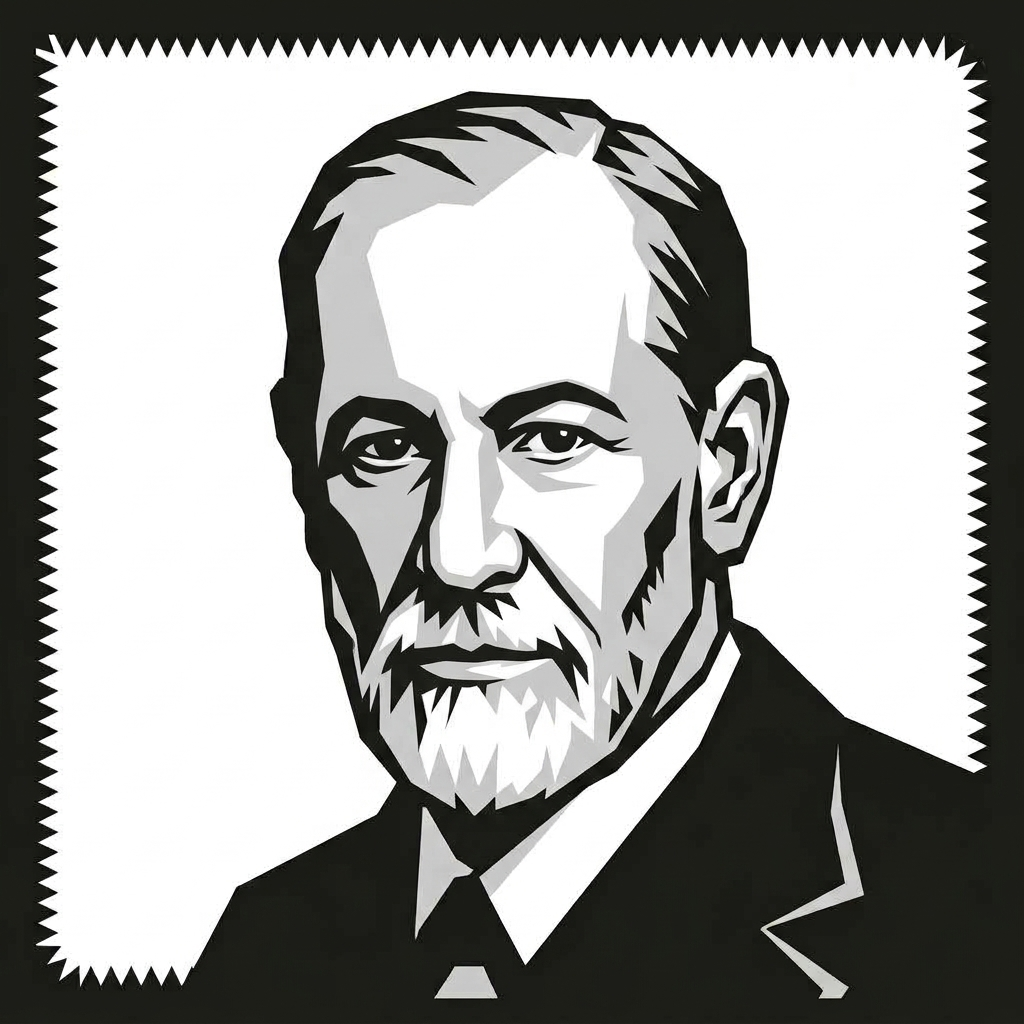
\includegraphics[width=0.85\textwidth, keepaspectratio]{freud.jpg}
                \\[0.1cm]
                \tiny\textit{\glqq Das Unbehagen in der Kultur\grqq}
            \end{tcolorbox}
        \end{column}
    \end{columns}
\end{frame}

\end{document}
